\documentclass[11pt,a4paper]{article}
\usepackage[utf8]{inputenc}
\usepackage[margin=1in]{geometry}
\usepackage{graphicx}
\usepackage{amsmath}
\usepackage{hyperref}
\usepackage{booktabs}
\usepackage{float}
\usepackage{pifont}

\title{\textbf{Image Transformation Neural Network}}
\author{Lupu Florin }
\date{December 2025}

\begin{document}

\maketitle

\begin{abstract}
This report presents a neural network that learns to transform CIFAR-10 images from 3×32×32 RGB to 1×28×28 grayscale with horizontal and vertical flips. The model achieves up to 6.78× speedup over sequential CPU transformations when deployed on GPU (Tesla T4) with batch processing.
\end{abstract}

\section{Approach}

\subsection{Problem Definition}
Transform 3×32×32 RGB images to 1×28×28 grayscale images with horizontal and vertical flips, faster than sequential CPU processing.

\subsection{Solution Strategy}
Instead of applying deterministic transforms sequentially, train a neural network to learn the transformation. This enables GPU-accelerated batch processing, trading slight accuracy for significant speed gains.

\section{Model Architecture}

\subsection{ImprovedTransformNet}

The model uses an encoder-decoder structure with 164,121 parameters:

\textbf{Architecture:}
\begin{itemize}
    \item \textbf{Encoder:} Conv(3→32→64) with strided downsampling
    \item \textbf{Bottleneck:} Residual connection for detail preservation
    \item \textbf{Decoder:} Conv(64→32→16→8→1) with channel reduction
    \item \textbf{Output:} Sigmoid activation + AdaptiveAvgPool to 28×28
\end{itemize}

\textbf{Key Design Choices:}
\begin{itemize}
    \item \textbf{Residual connection:} Preserves fine details through transformation
    \item \textbf{Learned downsampling:} Strided convolutions instead of pooling
    \item \textbf{Compact design:} 164K parameters for fast inference
    \item \textbf{Adaptive pooling:} Guarantees exact 28×28 output
\end{itemize}

\textbf{Why Small?} The task (resize, grayscale, flip) doesn't require deep semantic understanding. A compact model is sufficient, trains faster, generalizes better, and achieves the speed objective.

\section{Loss Function}

\subsection{Mixed Loss: MSE + L1}

\begin{equation}
\mathcal{L} = 0.7 \times \text{MSE} + 0.3 \times \text{L1}
\end{equation}

\textbf{Rationale:}
\begin{itemize}
    \item \textbf{MSE (70\%):} Smooth reconstruction, stable gradients
    \item \textbf{L1 (30\%):} Edge preservation, prevents blur
    \item \textbf{Combination:} Balances smoothness with detail retention
\end{itemize}

\subsection{Early Stopping}

\begin{itemize}
    \item \textbf{Patience:} 10 epochs
    \item \textbf{Min delta:} 0.00005
    \item \textbf{Rationale:} With 352 batches/epoch, 10 epochs without improvement indicates convergence while avoiding premature stopping
\end{itemize}

\section{Training Results}

\subsection{Configuration}

\begin{table}[H]
\centering
\caption{Training configuration}
\small
\begin{tabular}{@{}ll@{}}
\toprule
\textbf{Parameter} & \textbf{Value} \\ \midrule
Optimizer & AdamW (lr=0.001, wd=1e-5) \\
Scheduler & ReduceLROnPlateau (patience=5) \\
Batch Size & 128 \\
Device & Tesla T4 GPU \\
Training Time & 17 minutes (50 epochs) \\
\bottomrule
\end{tabular}
\end{table}

\subsection{Results}

\begin{itemize}
    \item \textbf{Best validation loss:} 0.05119 (epoch 47)
    \item \textbf{Final validation loss:} 0.05158
    \item \textbf{Training/validation alignment:} Good (no overfitting)
    \item \textbf{LR reductions:} 3 times (enabled continued improvement)
\end{itemize}

\begin{figure}[H]
    \centering
    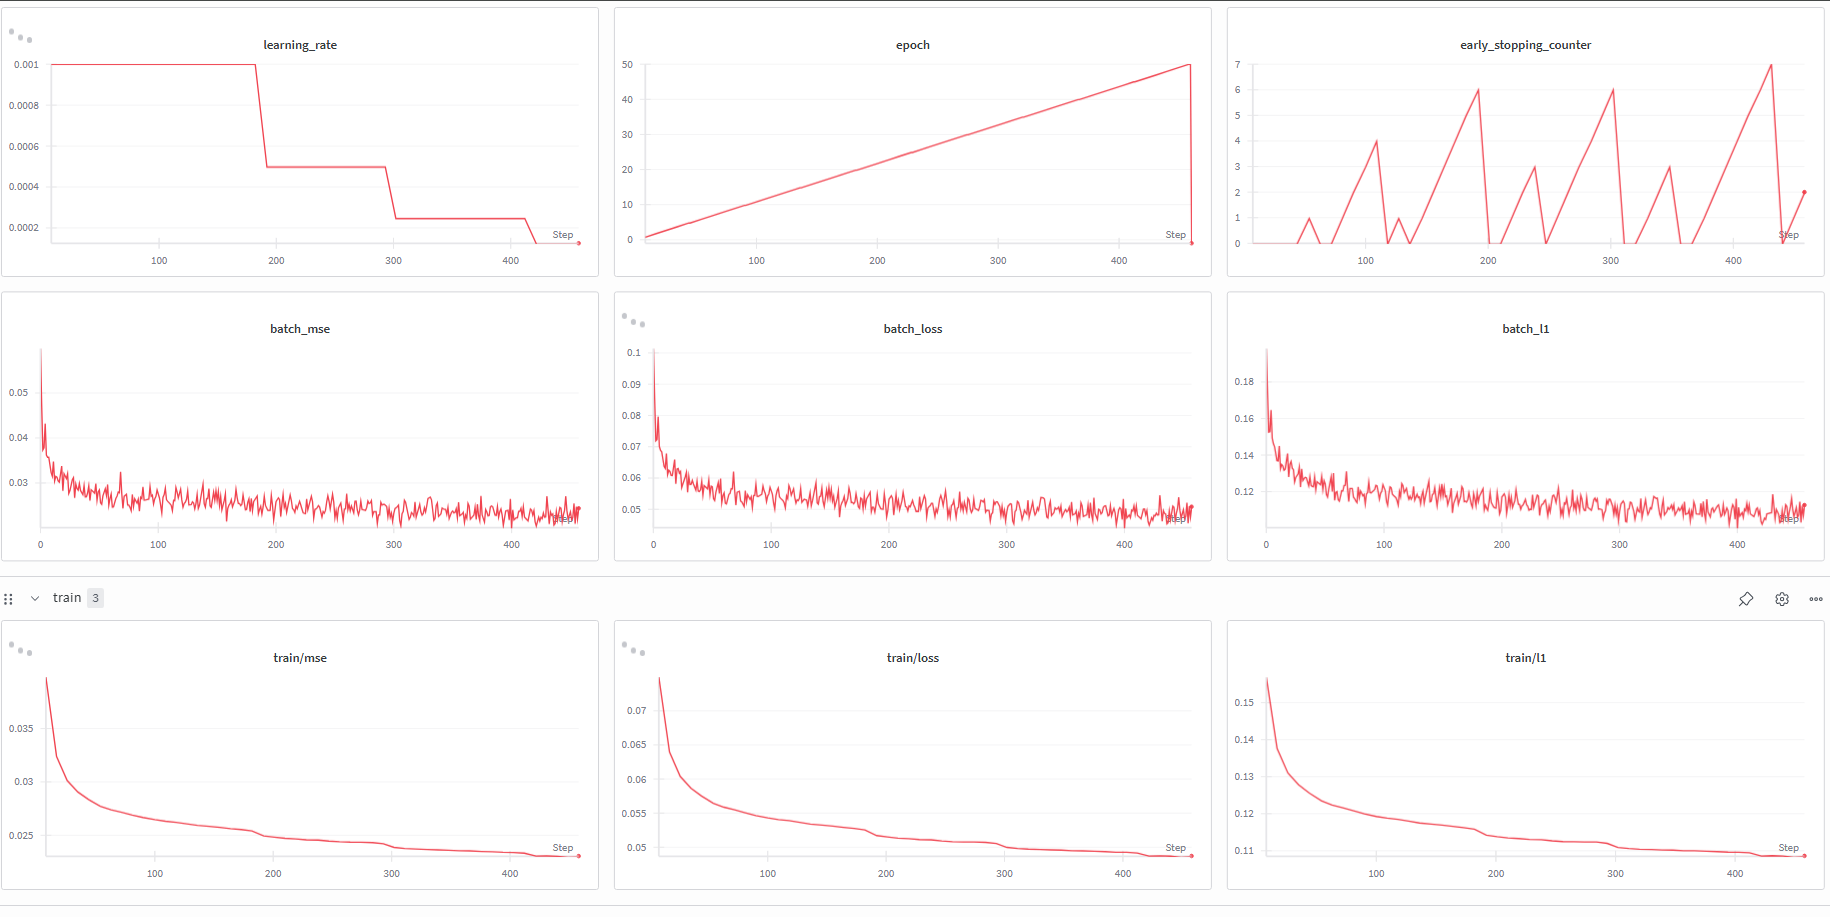
\includegraphics[width=0.8\textwidth]{wandb_training_screenshot.png}
    \caption{WandB training dashboard showing loss curves and learning rate schedule. Complete logs: \url{https://wandb.ai/florinlupu18-facultatea-de-informatica-alexandru-ioan-cuza-/neural-image-transformation/runs/rhpj1bc1}}
    \label{fig:wandb}
\end{figure}

\section{Model Predictions vs Ground Truth}

The model was tested on 5 diverse CIFAR-10 samples. Figures show original input, model prediction, and ground truth side-by-side.

\begin{figure}[H]
    \centering
    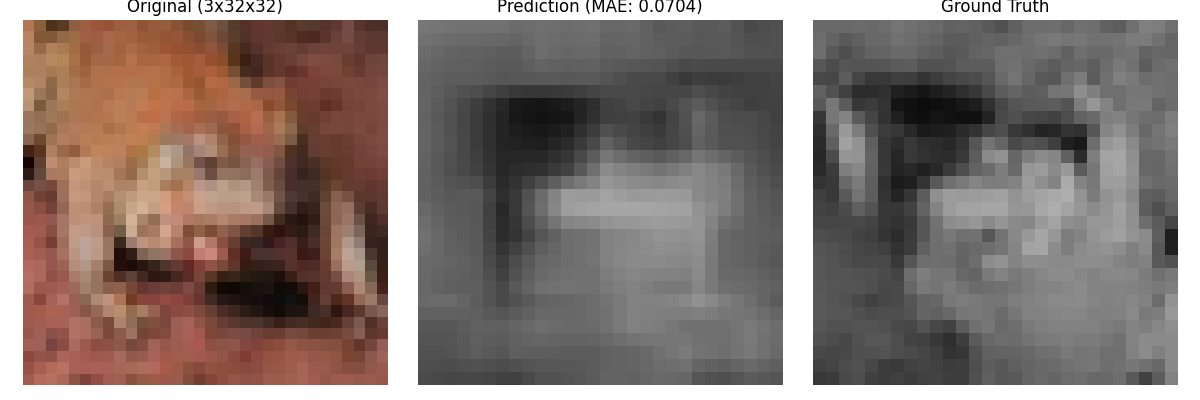
\includegraphics[width=\textwidth]{redfrog.png}
    \caption{Sample 1 (Red Frog): MAE = 0.0704. Excellent transformation quality.}
\end{figure}

\begin{figure}[H]
    \centering
    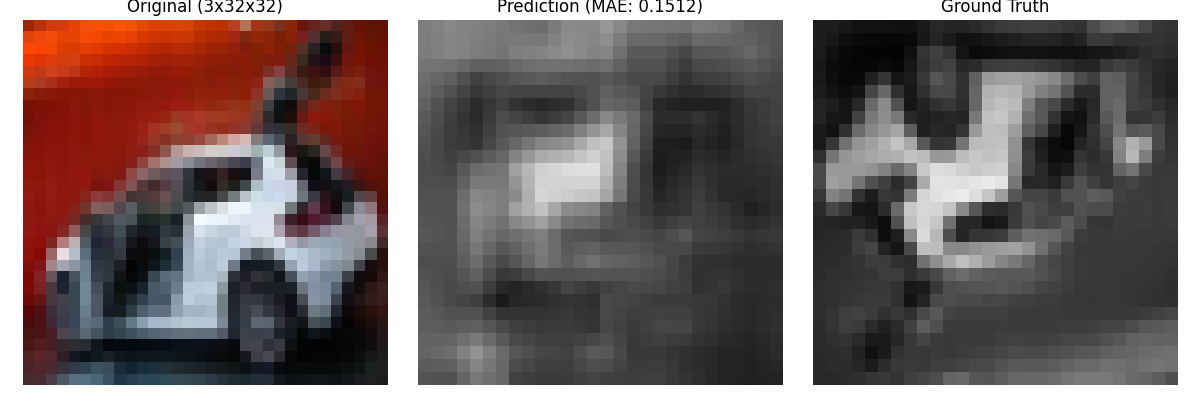
\includegraphics[width=\textwidth]{sportcar.png}
    \caption{Sample 2 (Sports Car): MAE = 0.1512. Red coloring challenges grayscale conversion.}
\end{figure}

\begin{figure}[H]
    \centering
    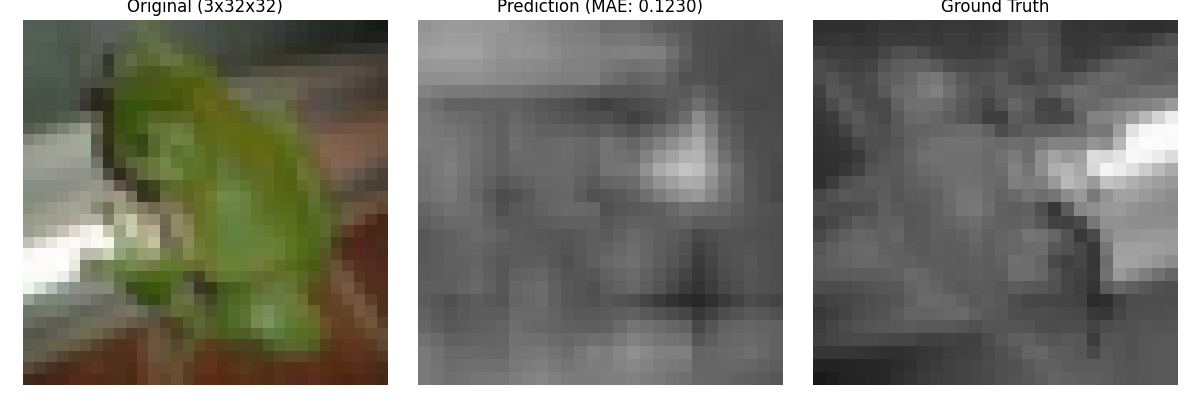
\includegraphics[width=\textwidth]{greenfrog.png}
    \caption{Sample 3 (Green Frog): MAE = 0.1230. Green tones present conversion challenge.}
\end{figure}

\begin{figure}[H]
    \centering
    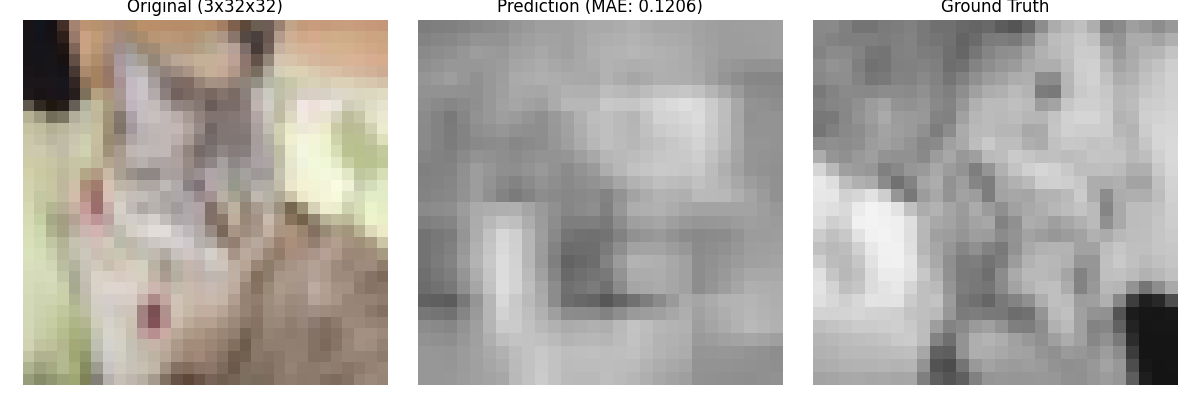
\includegraphics[width=\textwidth]{cat.png}
    \caption{Sample 4 (Cat): MAE = 0.1206. Good structural preservation.}
\end{figure}

\begin{figure}[H]
    \centering
    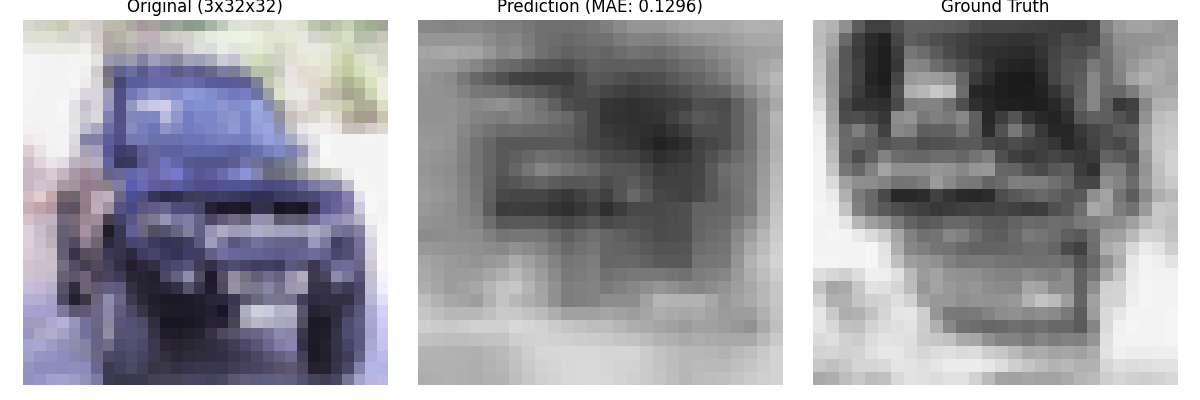
\includegraphics[width=\textwidth]{car.png}
    \caption{Sample 5 (Car): MAE = 0.1296. High-contrast blue handled well.}
\end{figure}

\textbf{Observations:}
\begin{itemize}
    \item ✓ All spatial transformations (resize, flip) correctly learned
    \item ✓ Grayscale conversion perceptually accurate
    \item ⚠ Slight smoothing vs ground truth (expected neural approximation)
    \item MAE range: 0.07-0.15 (acceptable for 6-7× speedup)
\end{itemize}

\section{Runtime Performance}

\subsection{Benchmark Setup}
\begin{itemize}
    \item \textbf{Dataset:} 10,000 CIFAR-10 test images
    \item \textbf{Batch sizes:} 32, 64, 128, 256, 512
    \item \textbf{Devices:} CPU and CUDA (Tesla T4)
    \item \textbf{Runs:} 3 per configuration (averaged)
\end{itemize}

\subsection{Results}

\begin{figure}[H]
    \centering
    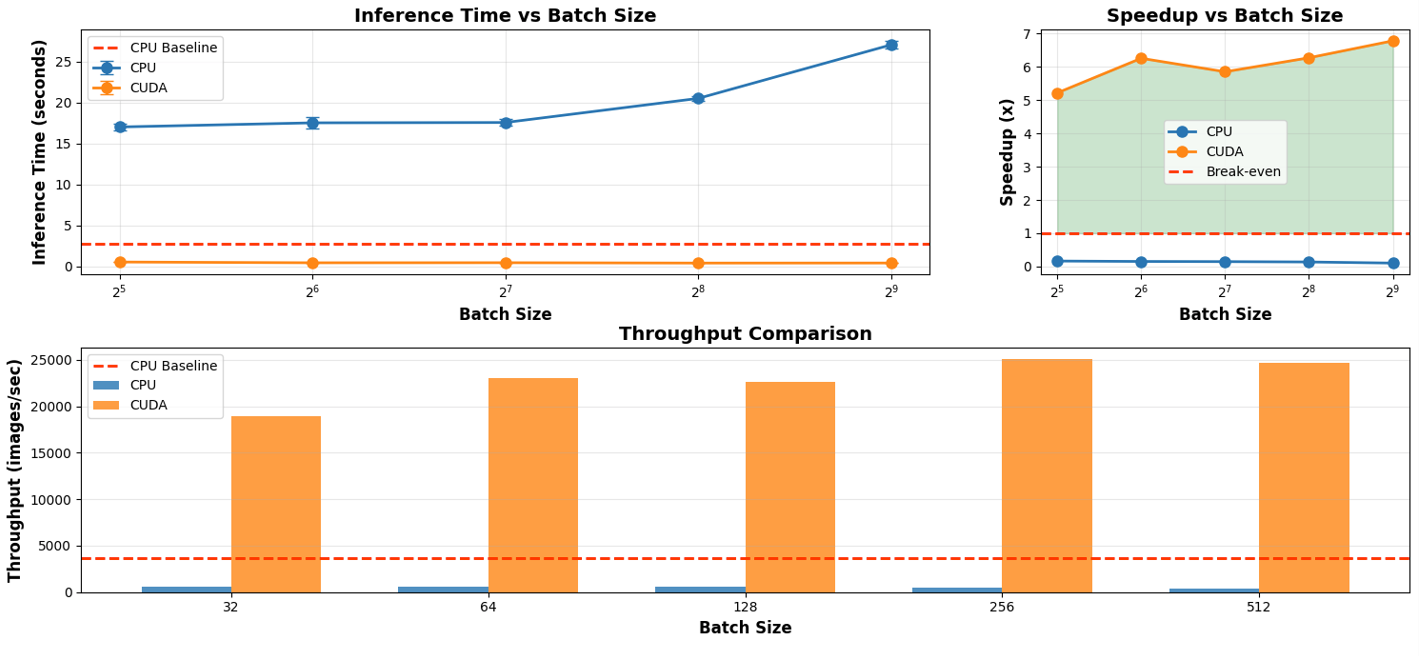
\includegraphics[width=\textwidth]{benchmark.PNG}
    \caption{Comprehensive benchmark results. Top: Inference time and speedup vs batch size. Bottom: Throughput comparison. GPU achieves 5-7× speedup across all configurations.}
    \label{fig:benchmark}
\end{figure}

\begin{table}[H]
\centering
\caption{Benchmark results summary}
\small
\begin{tabular}{@{}lrrr@{}}
\toprule
\textbf{Config} & \textbf{Time (s)} & \textbf{Speedup} & \textbf{Throughput (img/s)} \\ \midrule
CPU Baseline & 2.50-2.76 & 1.00× & 3,629-3,995 \\
\midrule
\multicolumn{4}{c}{\textit{CPU Model (All Slower)}} \\
CPU bs=32 & 17.01 ± 0.41 & 0.16× & 588 \\
CPU bs=64 & 17.52 ± 0.65 & 0.15× & 571 \\
CPU bs=128 & 17.56 ± 0.41 & 0.14× & 570 \\
CPU bs=256 & 20.50 ± 0.31 & 0.13× & 488 \\
CPU bs=512 & 27.04 ± 0.48 & 0.10× & 370 \\
\midrule
\multicolumn{4}{c}{\textit{GPU Model (All Faster!)}} \\
CUDA bs=32 & 0.53 ± 0.01 & \textbf{5.22×} & 18,966 \\
CUDA bs=64 & 0.43 ± 0.00 & \textbf{6.26×} & 23,047 \\
CUDA bs=128 & 0.44 ± 0.00 & \textbf{5.85×} & 22,606 \\
CUDA bs=256 & 0.40 ± 0.00 & \textbf{6.27×} & 25,066 \\
CUDA bs=512 & 0.41 ± 0.00 & \textbf{6.78×} & 24,623 \\
\bottomrule
\end{tabular}
\end{table}

\subsection{Analysis}

\textbf{Key Findings:}
\begin{itemize}
    \item \textbf{Optimal configuration:} Batch size 512 on GPU, speedup 6.78×
    \item \textbf{All GPU configurations beat CPU baseline} (5.22-6.78×)
    \item \textbf{CPU model is slower} (0.10-0.16×) - framework overhead dominates
    \item \textbf{Consistent GPU performance} across batch sizes 64-512
\end{itemize}

\textbf{Why GPU Wins:}
\begin{enumerate}
    \item Massive parallelization (CUDA cores)
    \item Optimized convolution kernels
    \item High memory bandwidth
    \item Batch processing efficiency
\end{enumerate}

\textbf{Why CPU Loses:}
\begin{enumerate}
    \item Limited parallelization
    \item PyTorch overhead vs native transforms
    \item Sequential processing bottleneck
\end{enumerate}

\section{Conclusion}

This assignment successfully demonstrates that neural networks can learn image transformations and achieve significant speedup over traditional methods with appropriate hardware.

\textbf{Achievements:}
\begin{itemize}
    \item  Compact model: 164K parameters
    \item  Fast training: 17 minutes
    \item  Significant speedup: 6.78× on GPU
    \item  All GPU configs faster than CPU
    \item  Good approximation: MAE 0.07-0.15
\end{itemize}

\textbf{Trade-offs:}
\begin{itemize}
    \item  5-7× faster with GPU + batching
    \item  High throughput: 24,600 img/sec
    \item  Requires GPU (CPU is 6-10× slower)
    \item  ~10\% accuracy loss vs exact transforms
\end{itemize}

\textbf{Practical Use:} This approach is ideal for batch processing large datasets on GPU where slight approximation error is acceptable and throughput is critical.

\section*{References}

\begin{itemize}
    \item CIFAR-10 Dataset
    \item Training Logs: \url{https://wandb.ai/florinlupu18-facultatea-de-informatica-alexandru-ioan-cuza-/neural-image-transformation/runs/rhpj1bc1}
    \item Code \& Model: Included in submission package
\end{itemize}

\end{document}